\documentclass{article}
\usepackage{CJKutf8}
\usepackage{indentfirst}
\usepackage{graphics}
\usepackage{epsfig}
\usepackage{graphicx}
\usepackage{amsmath}
\usepackage{amssymb}
\usepackage{listings}
\usepackage{hyperref}
\usepackage{color}
\usepackage{pgffor}
\usepackage[nottoc,numbib]{tocbibind}
\usepackage[toc,page]{appendix}
\definecolor{dkgreen}{rgb}{0,0.6,0}
\definecolor{gray}{rgb}{0.5,0.5,0.5}
\definecolor{mauve}{rgb}{0.58,0,0.82}

\lstset{frame=tb,
	language=C,
	aboveskip=3mm,
	belowskip=3mm,
	showstringspaces=false,
	columns=flexible,
	basicstyle={\small\ttfamily},
	numbers=none,
	numberstyle=\tiny\color{gray},
	keywordstyle=\color{blue},
	commentstyle=\color{dkgreen},
	stringstyle=\color{mauve},
	breaklines=true,
	breakatwhitespace=true,
	tabsize=3
}
\setlength{\parindent}{2em}
\renewcommand{\contentsname}{目录}
\renewcommand{\listfigurename}{插图目录}
\renewcommand{\listtablename}{表格目录}
\renewcommand{\refname}{参考文献}
\renewcommand{\abstractname}{摘要}
\renewcommand{\indexname}{索引}
\renewcommand{\tablename}{表}
\renewcommand{\figurename}{图}
\renewcommand{\appendixname}{附录}
%opening
\date{2016年11月}
\title{编译原理实验报告}
\author{何宜晖\\计算机46\\2140504137\\电信学院\\heyihui@stu.xjtu.edu.cn}

\begin{document}
\begin{CJK}{UTF8}{gkai}
%gkai gbsn
\begin{figure}
\centering
\includegraphics[width=0.6\linewidth]{/home/eli/Pictures/xjtu}
\end{figure}


\maketitle
\clearpage

\tableofcontents
\clearpage

\section{语法分析}
\subsection{实验目的}
\begin{enumerate}
	\item 强化对系统软件综合工程实现能力的训练
	\item 加强对词法分析原理、方法和基本实现技术的理解
\end{enumerate}

\subsection{实验内容}
用C语言或者其他的高级语言作为宿主语言完成C1语言的词法分析器的设计和实现。
%\setcounter{section}{0}
\subsection{实验要求}
\begin{enumerate}
\item 编写C0语言的词法分析器的源程序并调试通过。其中词法分析程序既可以自己手动去完成,也可以利用LEX自动生成。
\item 通过测试程序的验收; 
\item 实验报告按照提供的模板填写 
\end{enumerate}


\subsection{功能描述}
该程序要实现的是一个读程序的过程,从输入的源程序中,识别出各种类型的单词(基本保留字、标识符、常数、运算符、分隔符)。输出并打印各个单词的类型以及本身.\cite{chen2000}\cite{appel2004modern}\cite{louden2000}\cite{appel2006}.
我编写了几个简单的c0语言程序,解析结果在附录\ref{append}中

类型名按照实验指导书定义,部分未出现的,参照 ANSI C \cite{ansic}

分析部分,可以开启yylineao,用于打开自动记录行号\verb|%option yylineao|。
匹配到的词可以用\verb|yytext|直接获取。

主程序部分,\verb|yyin|将读取到的文件传送给lex。 \verb|yylex()| 则开始词法分析,每个匹配到的词,都会执行后面动作。\cite{levine1992lex}\cite{lesk1975lex}
\subsubsection{注释的跳过}\label{sec:com}
读到\verb|\\|我们就吃掉整行。
读到\verb|\*|我们进入注释程序\verb|comment()|. 一直读取,直到读到\verb|*/|为止,否则报错。

\subsection{程序结构描述}
程序使用lex编写,按指导书给出的状态转换图进行正则匹配,状态转移图如图\ref{fig:state}所示。

程序中设计了一个关键的打印函数 printToken, 该函数输入为当前识别的类型,输出为打印当前的行号,字符,以及类型。另一个函数是comment函数,用来判断当前注释进行的状态,如果注释出错,则需要报错,在章节\ref{sec:com}中已经详细解释了。另外则是主函数main,用于读取程序,启动yylex()程序解析。

具体lex的C语言实现,请见附录\ref{code},
使用lex分析C0程序的结果,请见附录\ref{append}.
\begin{figure}[!h]
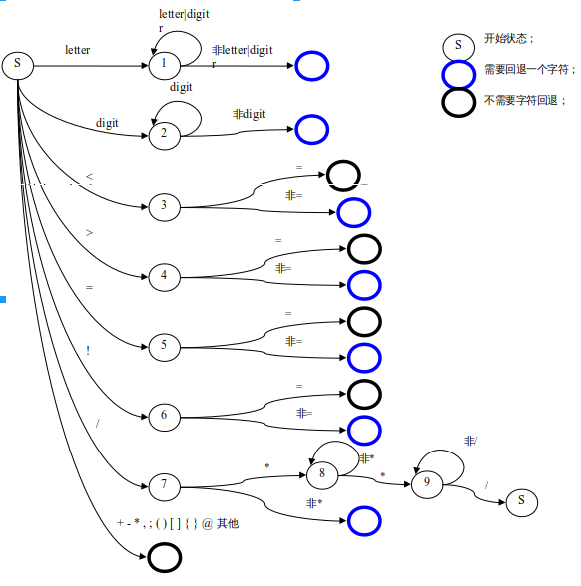
\includegraphics[width=\linewidth]{lex}
\caption{状态转换图}
\label{fig:state}
\end{figure}

\subsection{实验总结}
\begin{enumerate}
\item 你在编程过程中花时多少?我大概花了一个晚上。
\item  多少时间在纸上设计?花了半小时在纸上设计。
\item  多少时间上机输入和调试?3个小时左右。
\item  多少时间在思考问题?一个小时左右。
\item  遇到了哪些难题,你是怎么克服的? 实验中还是遇到了很多难题。首先是如何使用lex,经过仔细阅读参考书目lex\&yacc\ref{levine1992lex}, 让我了解了lex的基本用法。还有就是如何显示行号,如何获得当前的字符,我通过上网搜索了解到可以使用yylineao,yytext。以及如何解决有注释的问题,虽然实验指导书没有给出,我还是在参考书目中感悟到了解决方法\ref{levine1992lex}
\item  你对你的程序的评价?我的程序使用lex编写,token定义模仿标准的ANIS C。自己比较满意。
\item  你的收获有哪些?这次实验学会了使用lex,为后面利用yacc进行语法分析打下了坚实的基础。
\end{enumerate}

\clearpage
\section{语法分析}
\subsection{实验目的}
\begin{enumerate}
	\item 强化对系统软件综合工程实现能力的训练;
	\item 加强对语法分析原理、方法和基本实现技术的理解;
\end{enumerate}

\subsection{实验内容}
\begin{enumerate}
	\item 用C语言或者其他的高级语言作为宿主语言完成C0语言的词法分析器的设计和实现.
	\item 针对if语句的文法编写一个递归下降分析程序,输出结果为抽象语法树。注意,if语句文法中的表达式E采用四则运算表达式的文法;抽象语法树的格式自行设计,如果需要降低难度的话,也可用具体语法树而不用抽象语法树作为输出.
\end{enumerate}

\subsection{实验要求}
\begin{enumerate}
\item 编写C0语言的语法分析器的源程序并调试通过。其中语法分析程序既可以自己手动去完成,也可以利用YACC自动生成。
\item 通过测试程序的验收; 
\item 实验报告按照提供的模板填写:
\end{enumerate}

\subsection{功能描述}
该程序要实现的是一个读程序的过程,从输入的源程序中生成一颗抽象语法树\cite{chen2000}\cite{appel2004modern}\cite{louden2000}\cite{appel2006}.,并将结果保存为xml。

我编写了一些简单的c0语言程序,输出结果见附录\ref{app}.

大部分语法,终结符非终结符的定义,我都是参照实验指导书给出的c0语法如下。部分语法参照 ANSI C \cite{ansic}
\begin{verbatim}
    program→ { var-declaration | fun-declaration }
        var-declaration→ int ID { , ID }    
        fun-declaration→ ( int | void ) ID ( params ) compound-stmt
        params → int ID { , int ID } | void | empty
        compound-stmt→ { { var-declaration } { statement } }
        statement→ expression-stmt∣compound-stmt ∣if-stmt ∣while-stmt 
        |return-stmt 
        expression-stmt→ [ expression ] ; 
        if-stmt→ if( expression ) statement [ else statement ]
        while-stmt→ while( expression ) statement 
        return-stmt→ return [ expression ] ;
        expression→ ID = expression | simple-expression
        simple-expression→ additive-expression [ relop additive-expression ]
        relop → < | <= | > | >= | == | != 
        additive-expression→ term [( + | - ) term ]
        term→ factor [ ( * | / ) factor ]
       factor→ ( expression )| ID | call | NUM
       call→ ID( args ) 
       args→ expression { , expression } | empty
       ID →…	;参见C语言标识符定义
       NUM →… ;参见C语言数的定义
\end{verbatim}
\subsection{程序结构描述}
\subsubsection{ifelse}
本程序有一个\textbf{移进归约冲突}:
\begin{verbatim}
  IF '(' expression ')' statement _ ELSE statement
\end{verbatim}
由于yacc默认的优先级是从上到下,只需要把if写在if else前面,这个冲突可以默认被消解。
\subsubsection{双目运算}
双目运算$+,-,*,/$ 需要具有左结合性,否则会产生歧义,并且乘除应当比加减先结合。具体到yacc如下:
\begin{verbatim}
%left PLUS MINUS
%left STAR SLASH
\end{verbatim}
\subsubsection{单目运算}
单目运算+-,结合紧密型应当比乘除高,然而在前面已经定义了结合紧密性低于乘除,所以需要在单目运算中单独处理,具体到yacc时,使用prec语法, 临时更换其结合紧密性。
\begin{verbatim}
additive_expression
    ...
    ...
    | PLUS additive_expression %prec STAR {...}
    | MINUS additive_expression %prec STAR {...}
\end{verbatim}
\subsubsection{$++,--$}
这是在c,c0,c++等语言中的特殊语法。如果在词法分析时,只单个提取+,-。后面是无法区分--i与-(-i)的,会有\textbf{归约-归约冲突}。故需要定义两个单独的token,与+,-区别开来。
\begin{verbatim}
%token INC_OP DEC_OP
\end{verbatim}
在词法分析时,就要单独识别:
\begin{verbatim}
"++"				{return INC_OP; }
"--"				{return DEC_OP; }
\end{verbatim}
在语法分析时,就能轻松区别开了:
\begin{verbatim}
unary_expression 
    : INC_OP ID {...}
    | DEC_OP ID {...}
    | postfix_expression {...}
    ;

postfix_expression
    : ID INC_OP {...}
    | ID DEC_OP {...}
    ;
\end{verbatim}
\subsubsection{$V_T \& V_N$}
终结符直接用string表示,非终结符用语法树的节点表示。
\begin{lstlisting}[language=c]
%union {
    char* str;
    struct treeNode * ast;
}
\end{lstlisting}
在yacc中,需要分别定义类型:
\begin{verbatim}
%type<ast> atree program ...
%type<str> relop declaration_specifiers 
\end{verbatim}

\subsubsection{Abstract Tree}
\textbf{语法树节点},便于输出打印, child便于递归打印:
\begin{lstlisting}[language=c]
struct treeNode{
    struct treeNode *child[MAXCHILD];
    char* nodeType;
    char* string;
    char* value;
    char* dataType;
    int lineNo;
    int Nchildren;
};
\end{lstlisting}


\textbf{递归生成语法树},在yacc中 \verb|$$,$1,$2,$3|可以用来返回指针,
以及获得下一级的指针。
yacc会递归地,先按照需求计算对应位置非终结符的返回值。
使用方法如下:
\begin{verbatim}
params
    : params_list {$$=$1;}
    | VOID {$$ = newnode(yylineno,"params", none, none, "VOID",  0);}
    ;
\end{verbatim}

而newnode,是用来将节点穿起来的函数,利用了yacc递归的性质:
\begin{lstlisting}[language=c]
struct treeNode * newnode(int lineNo, char* nodeType, char* string, char* value, char* dataType, int Nchildren, ...){
    struct treeNode * node = (struct treeNode*) malloc(sizeof(struct treeNode));
    node->nodeType = nodeType;
    node->string = string;
    node->value = value;
    node->dataType = dataType;
    node->lineNo = lineNo;
    node->Nchildren = Nchildren;
    va_list ap;
    int i;
    va_start(ap, Nchildren);
    for (i=0;i<Nchildren;i++){
        node->child[i]=va_arg(ap, struct treeNode *);
    }
    va_end(ap);
    return node;
}
\end{lstlisting}

\textbf{打印语法树},需要使用\textbf{拓广文法}。
单独设定一个非终结符atree在程序开始,它没有任何语法意义,仅仅是为了开始节点有区分性,用来打印语法树。

\begin{verbatim}
%start atree
%%
atree:program {printNode($1);}
\end{verbatim}

\begin{lstlisting}[language=c]
void printNode(struct treeNode* node){
    printf("%s<Tree lineNo=\"%d\" nodeType=\"%s\" string=\"%s\" value=\"%s\" dataType=\"%s\">\n", 
        indent,
        node->lineNo,
        node->nodeType,
        node->string,
        node->value, 
        node->dataType);
    int i;
    if (node->Nchildren > 0){
        printf("%s<Child>\n", indent);
        incIndent();
        for (i=0;i<node->Nchildren;i++){
            printNode(node->child[i]);
        }
        decIndent();
        printf("%s</Child>\n", indent);
    }
    printf("%s</Tree>\n", indent);
}
\end{lstlisting}

\subsubsection{程序的缺陷}
本程序有一个缺陷,就是打印行号时,会打印出匹配到的非终结符的最后一行的行号,而不是样例中给出的第一行的行号。这是自下而上分析的栈读取的特性导致的,我暂时还不知道怎么解决。

\subsubsection{程序代码}
程序代码,见附录\ref{coder}

语法分析结果,见附录\ref{app}
\subsection{实验总结}
\begin{enumerate}
\item 你在编程过程中花时多少?我大概花了两个晚上。
\item  多少时间在纸上设计?花了一小时在纸上设计。
\item  多少时间上机输入和调试?6个小时左右。
\item  多少时间在思考问题?3个小时左右。
\item  遇到了哪些难题,你是怎么克服的? 实验中还是遇到了很多难题。首先是如何使用yacc,经过仔细阅读参考书目lex\&yacc \cite{levine1992lex}, 让我了解了yacc的基本用法。其他大部分问题都是通过上网查找相关资料解决的,具体困难和解决可以参考实验报告前面部分
\item  你对你的程序的评价?我的程序使用yacc和lex编写,token定义模仿标准的ANIS C。只有一个shift/reduce冲突,自己非常满意。
\item  你的收获有哪些?这次实验学会了使用yacc,以及如何将lex和yacc配合使用。这次实验后,我对编译原理产生了浓厚的兴趣。
\end{enumerate}

\clearpage
{\small
	\bibliographystyle{ieee}
	\bibliography{he16yacc}
}
\clearpage

\appendix
\section{lex code}\label{code}
\lstinputlisting[language=c]{../c-compiler/q1.l}

\clearpage
\section{lex results}\label{append}

\foreach \n in {orig.c,simple.c,test.c,test2.c,testlex.c,testparser.c}{
	 $c_0$ 语言文件 \n
	\lstinputlisting[language=c]{../c-compiler/test/\n}
	$c_0$ 语言文件 \n 的输出
	\lstinputlisting[language=xml]{../c-compiler/test/\n.lex.xml}
}

\clearpage
\section{yacc code}\label{coder}

yacc 文件:q2.y
\lstinputlisting[language=c]{../c-compiler/q2.y}

yacc文件对应的lex文件:q2.l
\lstinputlisting[language=c]{../c-compiler/q2.l}

\clearpage
\section{yacc results}\label{app}

\foreach \n in {orig.c,simple.c,test.c,test2.c,testlex.c,testparser.c}{
	 $c_0$ 语言文件 \n
	\lstinputlisting[language=c]{../c-compiler/test/\n}
	$c_0$ 语言文件 \n 的输出
	\lstinputlisting[language=xml]{../c-compiler/test/\n.xml}
}

\end{CJK}
\end{document}
